\chapter{Early models of an atom}\label{c3}
We will review the models of an atom proposed before the development of quantum
mechanics. The purpose of this chapter is less to give an account of the 
historical development and more to illustrate how conceptually simple 
experiments and relatively straightforward application of the laws of physics 
proved these models to be inadequate.

\section{Thomson's model}\label{c3s1}
Sir J. J. Thomson proposed a model of an atom as a uniformly distributed 
positive charge in which negatively charged electrons are studded. The atom as
a whole was thought to be impenetrable. This was very much in line with the 
ideas of continuous solids and fluids of the late nineteenth century. The only
way to find out if matter was indeed continuous was to bombard it with high
energy particles and check how many of them make it to the other side. This
is exactly what Geiger and Marsden in a series of experiments between 1908 and
1913. Geiger's first experimenti \cite{geiger1908scattering} consisted of 
bombarding alpha particles on a thin gold foil and checking how many of them 
reach the detector at the end of a $2$ m long evacuated glass tube. The alpha 
particles are collimated before they enter the tube. In the absence of the foil 
they create a sharply defined image of the slit. When a little air was admitted 
the alpha particles collided with the air molecules and caused the image to 
blur. When the tube was evacuated again and a gold foil fitted midway between 
the collimating slit and the detector, a blurred image was formed. If the matter
were indeed continuous then no alpha particle should have made it to the other
side. Further, there was no qualitative difference between the image caused by a
few gas particles and a solid foil indicating that the `solid' foil was 
probably full of pores. Geiger collaborated with Marsden in his next experiment,
published \cite{gegier1909diffuse} in 1909, to prove that some alpha particles,
roughly $1$ ind $8000$ were scattered by the gold foil by an angle more than
$90^\circ$. This suggested that although the `solid' gold foil was largely 
porous, it did have a few very strong scattering centres. Since the alpha
particles are positively charged, the scattering centres too must have a 
positive charge. Geiger did another experiment \cite{geiger1910scattering} in 
the following year from which he concluded that the most probable angle of
deflection is directly proportional to the foil's thickness, atomic mass of
the foil's metal and with the speed of alpha particles. He also found that the
only a very few particles are scattered by more than $90^\circ$. These 
experiments proved that the Thomson's model was not correct and Rutherford 
proposed \cite{rutherform1911scattering} the nuclear model of an atom. It 
consisted of a tiny, positively charge nucleus and the electrons are in the 
rest of region, largely vacuous.

Sir J. J. Thomson, the originator of the eponymous model, was also the 
discoverer of electrons, which he called `corpuscules'. He was aware that 
they are far lighter than the hydrogen atom. Before we discuss the Rutherford
model in greater details let us analyse Thomson's model to show that it cannot
explain the large scattering observed in Geiger and Marsden's experiments. 
Consider the collision between two particles of mass $m_1$ and $m_2$. Let their
initial velocities be $v_1$ and $v_2 = 0$ and their final velocities be 
$v_1^\prime$ and $v_2^\prime$. Assume a head-on elastic collision. The 
conservation of momentum requires
\begin{equation}\label{c3s1e1}
m_1v_1 + 0 = m_1v_1^\prime + m_2v_2^\prime.
\end{equation}
Conservation of kinetic energy gives
\begin{equation}\label{c3s1e2}
m_1v_1^2 + 0 = m_1{v_1^\prime}^2 + m_2{v_2^\prime}^2.
\end{equation}
In these equations, $v_1$ is known and we want to express the final velocities
in terms of it. From \eqref{c2s1e1},
\begin{equation}\label{c3s1e3}
v_2^\prime = \frac{m_1}{m_2}(v_1 - v_1^\prime).
\end{equation}
Substituting this in \eqref{c3s1e2} we get the quadratic
\begin{equation}\label{c3s1e4}
(m_1 + m_2){v_1^\prime}^2 - 2m_1v_1v_1^\prime + (m_1 - m_2)v_1^2 = 0
\end{equation}
whose solutions are
\begin{equation}\label{c3s1e5}
v_1^\prime = \frac{m_1 \pm m_2}{m_1 + m_2}v_1.
\end{equation}
The solution with the plus sign indicates a situation in which the collision
has not happened for the final velocity is identical with the initial one. That
is not true. Therefore,
\begin{equation}\label{c3s1e6}
v_1^\prime = \frac{m_1 - m_2}{m_1 + m_2}v_1
\end{equation}
and hence
\begin{equation}\label{c3s1e7}
v_2^\prime = \frac{2m_1}{m_1 + m_2}v_1.
\end{equation}
It was known that the alpha particle was far more heavier than the electron.
That is $m_1 \gg m_2$ so that $v_2^\prime \approx 2v_1$. The alpha particle
loses a momentum $\Delta p_1 = 2m_2v_1$. If this loss is accompanied by a 
deflection by an angle $\theta$ then
\begin{equation}\label{c3s1e8}
\tan\theta = \frac{\Delta p_1}{p_1} = \frac{2m_2}{m_1}.
\end{equation}
Since $m_2$ is far smaller than $m_1$, $\theta$ is very close to zero. Thus,
a collision with an electron cannot explain the large-angle deflection of an
alpha particle.

If the electrons cannot deflect alpha particles can the uniform positive
charge distribution of the rest of the atom? The electric field of a uniformly
distributed charge distribution is found using Gauss's law,
\begin{equation}\label{c3s1e9}
\oint_S \vec{E}.\hat{n}da = \frac{\epsilon_0}{Q},
\end{equation}
where $Q$ is the charge enclosed by the surface $S$ and $\epsilon_0$ is the 
permittivity of free space. Let $R$ be the radius of an atom, assumed spherical.
If $r < R$,
\[
E\cdot 4\pi r^2 = \frac{1}{\epsilon_0} \rho_e \frac{4\pi}{3}r^3
\]
where $\rho_e$ is the charge density so that
\[
E = \frac{1}{3\epsilon_0}\rho_e r.
\]
If there are $Z$ electrons then to keep the atom electrically neutral we need
a charge $Ze$ distributed uniformly in a volume $4\pi R^3/3$ or
\begin{equation}\label{c3s1e10}
\rho_e = \frac{3Ze}{4\pi R^3}
\end{equation}
so that the electric field is
\begin{equation}\label{c3s1e11}
\vec{E} = \frac{Ze}{4\pi\epsilon_0}\frac{r}{R^3}\hat{r},
\end{equation}
$\hat{r}$ being the unit vector in the radial direction. This expression is
true for all points $r \le R$. Clearly, the field is maximum at the surface of
the atom and the maximum force experienced by the alpha particle is when it is
just that the surface. Since the charge on the alpha particle is $2e$, it is
\begin{equation}\label{c3s1e12}
\vec{F} = \frac{2Ze^2}{4\pi\epsilon_0}\frac{1}{R^2}\hat{r}.
\end{equation}
Let us further assume that the force makes is most impact when the alpha 
particle is in a segment of length $L = 2R$ of the tangent at the point it
touches the spherical atom. Since the collision is assumed to be elastic, the
magnitude of velocity does not change, only its direction changes. A particle
with initial speed $v_1$ takes a time $\delta t = L/v_1$ to cross the segment of
maximum impact. Therefore, the impulse felt by the alpha particle is $F\delta t$
, which is also the change in its momentum. Thus,
\begin{equation}\label{c3s1e13}
\Delta p =\frac{2Ze^2}{4\pi\epsilon_0}\frac{1}{R^2}\frac{2R}{v_1}
\end{equation}
where we have used the fact that $L = 2R$. The angle of deflection is again
estimated using \eqref{c3s1e8} as
\begin{equation}\label{c3s1e14}
\tan\theta = \frac{Ze^2}{\pi\epsilon_0 R m_1v_1^2}.
\end{equation}
For a gold foil $Z = 79$. If we assume that the speed of the incident alpha
particles if $2 \times 10^7$ ms${}^{-1}$ then once again we get the same result 
that $\theta$ is very close to zero.

\section{Rutherford's model}\label{c3e2}
We mentioned about Geiger and Marsden's experiments that gave an experimental
proof against the Thomson's model. The large-angle scattering of a few alpha
particles led Rutherford to conjecture that the positive charge of the atom
is concentrated in a tiny nucleus. We will describe his model first proposed in
1911 \cite{rutherform1911scattering}. The scattering process is depicted in
figure \ref{c3f1} taken from \cite{rutherform1911scattering}. An alpha particle
approaches an atom in the direction $PO$ and is deflected in the direction 
$OP^\prime$.
\begin{figure}
\begin{center}
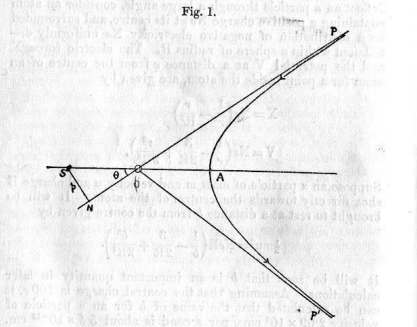
\includegraphics{rutherford-scattering}
\caption{Schematic diagram of Rutherford scattering}\label{c3f1}
\end{center}
\end{figure}
Rutherford assumed that the entire positive charge is concentrated in a point-
like nucleus at point $S$. Since the interaction between the nucleus and the
alpha particle is electrostatic, the trajectory is a hyperbola $PAP^\prime$ with
$S$ as its external focus. The point $O$ is chosen as the origin and the lines
$OP$ and $OP^\prime$ are its asymptotes. The line $SN$ is prependicular to the
asymptote and let its length be $p$. Let us further assume that the length of
the segment $OA$ is $q$. Then the equation of the hyperbola is
\begin{equation}\label{c3s2e1}
\frac{x^2}{q^2} - \frac{y^2}{p^2} = 1.
\end{equation}
This is because of the property of the hyperbola that the perpendicular distance
from a focus to either asymptote is the semi-minor axis $p$. Therefore, the
eccentricity is
\begin{equation}\label{c3s2e2}
\varepsilon = \sec\theta.
\end{equation}
Refer to the figure \ref{c3f2} taken from Wikipedia.
\begin{figure}
\begin{center}
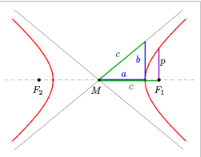
\includegraphics{hyperbola}
\caption{$x^2/a^2 - y^2/b^2 = 1$ from Wikipedia}\label{c3f2}
\end{center}
\end{figure}
Let $\vec{V}$ be the velocity of the alpha particle at $P$ and $\vec{v}$ be the
velocity at point $A$. Since the angular momentum is conserved in an 
electrostatic interaction,
\begin{equation}\label{c3s2e3}
pV = rv,
\end{equation}
where $r$ is the length of the segment $SA$. Note that both angular momenta are
taken around the point $S$ and \emph{not} the origin $O$. If the nucleus at $S$
carries a charge $Ze$ then the potential energy of the alpha particle with
charge $2e$ at point $A$ is
\[
\frac{2Ze^2}{r}
\]
so that by energy conservation we have
\begin{equation}\label{c3s2e4}
\frac{1}{2}mV^2 = \frac{1}{2}mv^2 + \frac{2Ze^2}{r}.
\end{equation}
Therefore,
\[
v^2 = V^2 - \frac{4Ze^2}{mr}
\]
or
\begin{equation}\label{c3s2e5}
v^2 = V^2\left(1 - \frac{b}{r}\right),
\end{equation}
where
\begin{equation}\label{c3s2e6}
b = \frac{4Ze^2}{mv^2}.
\end{equation}
$b$ is the closest distance at which an alpha-particle with energy $mV^2/2$
can approach a point nucleus with charge $Ze$. At this distance its entire 
kinetic energy is converted to electrostatic potential energy. From figures
\ref{c3f1} and \ref{c3f2} it is clear that the length of the segment $OA$ is
$p\cot\theta$ so that the length of $SA$ is
\begin{equation}\label{c3s2e7}
r = p\csc\theta + p\cot\theta = p\frac{1 + \cos\theta}{\sin\theta} =
p\frac{\cos\theta/2}{\sin\theta/2} = p\cot\frac{\theta}{2}.
\end{equation}
From equation \eqref{c3s2e3}
\[
V = \frac{rv}{p}.
\]
Substitute it in \eqref{c3s2e5} to get
\begin{equation}\label{c3s2e8}
v^2 = \frac{r^2v^2}{p^2}\frac{r - b}{r} \Rightarrow p^2 = r(r - b).
\end{equation}
Use \eqref{c3s2e7} for $r$ to get
\begin{equation}\label{c3s2e9}
p^2 = p\cot\frac{\theta}{2}\left(p\cot\frac{\theta}{2} - b\right)
\end{equation}
from which we get
\[
p^2 = p^2\cot^2\frac{\theta}{2} - bp\cot\frac{\theta}{2} \Rightarrow
bp\cot\frac{\theta}{2} = p^2\frac{cos\theta}{\sin^2(\theta/2)} \Rightarrow
b = 2p\frac{\cos\theta}{\sin\theta}
\]
or
\begin{equation}\label{c3s2e10}
b = 2p\cot\theta.
\end{equation}
The angle of deviation $\phi$ is the angle $POP^\prime$ in figure \ref{c3f1}.
$\angle POA = \angle AOP^\prime = \angle SON = \theta$ so that
\begin{equation}\label{c2s2e11}
\phi = \pi - 2\theta
\end{equation}
so that equation \eqref{c3s2e10} can be written as
\begin{equation}\label{c3s2e12}
\cot\left(\frac{\phi}{2}\right) = \frac{2p}{b}.
\end{equation}
Consider a pencil of alpha particles falling normally on the metal foil of
thickness $t$. Let $n$ be the number of atoms per unit volume of the material.
If the radius of an atom is $R$ then `cross sectional area' of the atom is
$\pi R^2$. A cylinder of this `base area' and height $h$ will have $nt\pi R^2$
number of sites where collisions can happen. The probability $P$ of an alpha
particle entering an atom within distance $p$ of its centre is
\begin{equation}\label{c3s2e13}
P = nt \pi p^2
\end{equation}
and the probability that it enters in an annulus of radii $p$ and $p + dp$ is
\begin{equation}\label{c3s2e14}
dP = 2nt\pi pdp.
\end{equation}
From equation \eqref{c3s2e12}
\begin{equation}\label{c3s2e15}
dp=-\frac{b}{4}\csc^2\left(\frac{\phi}{2}\right).
\end{equation}
Substituting \eqref{c3s2e12} and \eqref{c3s2e15} in \eqref{c3s2e14}, we get
\begin{equation}\label{c3s2e16}
dP = -nt\pi \frac{b^2}{4}\csc^2\left(\frac{\phi}{2}\right)
\cot\left(\frac{\phi}{2}\right).
\end{equation}
The probability of finding an alpha particle deflected between angles $\phi_1$
and $\phi_2$ is
\begin{equation}\label{c3s2e17}
P(\phi_1, \phi_2) = \int_{\phi_1}^{\phi_2}dP = \frac{\pi}{4}ntb^2\left(
\cot^2\left(\frac{\phi_1}{2}\right) - \cot^2\left(\frac{\phi_2}{2}\right)\right)
\end{equation}
If $F$ is the incident flux of the alpha particles then the number of particles
deflected between $\phi$ and $\phi + d\phi$ are $|FdP|$, where $dP$ is given 
by \eqref{c3s2e16} and we have used the modulus to ensure that the number of
particles is always a positive quantity. These particles land on the detector in
an annular region. The inner radius of this region is $s\sin\phi$ where $s$ is
the distance of any point on it from the centre of the incident pencil. The
circumference of the annulus is $2\pi r\sin\phi$ and the area of the annular
ring is $2\pi r\sin\phi d\phi$. Therefore, the number of particles deflected
between angles $\phi$ and $\phi + d\phi$ and and landing \emph{per unit area of 
the detector} is
\begin{equation}\label{c3s2e18}
N(\phi) = \Big|\frac{FdP}{2\pi s^2\sin\phi d\phi}\Big| = 
\frac{Fnt b^2\csc^2(\phi/2)\cot(\phi/2)}{8s^2\sin\phi}.
\end{equation}
Writing the denominator in terms of half angles we get
\begin{equation}\label{c3s2e19}
N(\phi) = \frac{Fntb^2}{16s^2}\csc^4\left(\frac{\phi}{2}\right).
\end{equation}
From equation \eqref{c3s2e6} we have
\begin{equation}\label{c3s2e20}
N(\phi) = \frac{FntZ^2e^4}{m^2v^4s^2}\csc^4\left(\frac{\phi}{2}\right).
\end{equation}
Thus, $N(\phi)$ is
\begin{enumerate}
\item directly proportional to $\csc^4(\phi/2)$;
\item directly proportional to the thickness $t$ of the foil;
\item directly proportional to the square of the atomic number $Z$ of the 
scatterer;
\item inversely proportional to the square of the kinetic energy of the incident
alpha particles. 
\end{enumerate}
Geiger and Marsden's experiments \cite{geiger1913lxi} showed that these
predictions are correct thereby putting the nuclear model of an atom on a firm
footing.

Rutherford's model and Geiger-Marsden's experiments showed that the atoms have
a very small nucleus where all the positive charge resides. It did not tell 
anything about the electrons. Either the electrons are smeared as a continuous
distrubution throughout the atom or that the electrons move around the nucleus
like planets around the sun. The former was ruled out because the even the
Thomson model had them as `corpuscules'. Since the entire positive charge is
concentrated in the nucleus, it is impossible for the electrons to remain
stationary as in Thomson's model. Therefore, the only option left was to assume
them to go aroud the nucleus. However, a charge going around a nucleus undergoes
an accelerated motion and radiates energy at the rate \cite[equation (20-44)]{
reitz2009foundations}
\begin{equation}\label{c3s2e21}
P_r = \frac{2}{3}\frac{e^2}{4\pi\epsilon_0}\frac{a^2}{c^3},
\end{equation}
where $a$ is its acceleration and $c$ is the velocity of light. This continuous
loss of energy will force the electron to spiral down and fall into the nucleus.
Thus, although Rutherford's model conclusively showed the existence of a nucleus
it could not account for the motion of electrons.

\section{Bohr's model}\label{c3s3}
The greatest deficiency in Rutherford's model was the radiative loss of 
accelerating electrons. Even if, for some reason, the radiative loss was 
suspended, the model could not account for the spectra of elements. Before we 
get to the details of the Bohr model, let us digress to understand emission
and absorption spectra.

\subsection{Absorption and Emission spectra}
The simplest spectrum that we have seen is that produced by a prism. When white
light is shone on a prism, it is split into seven colours. In a laboratory, the
white light is let from a narrow slit and one can observe seven slits, each one
of a different colour, from the other side. This is called a spectrum of white
lights. It consists of brightly coloured lines on a dark background and is 
called an emission spectrum.

Now place a beaker of water on the side from which we are seeing the spectrum.
The spectrum will be undisturbed, all seven colours will be seen. However, when
you add potassium permanganate to the beaker, the water turns purple and 
simultanuously the green line disappears. The `green' light is absorbed and that
is why the water appears purple. This is an absorption spectrum. 

Spectra of both kinds are signatures of the atoms or molecules that cause them.
In fact, the element Helium was first observed in the solar spectrum and then 
discovered on the earth.

The spectrum of Hydrogen atom is in the form of sharp lines and the greatest
triumph of Bohr model was in explaining why it is so.

\subsection{Bohr's postulates}
Bohr postulated \cite{bohr1913constitution} that the electron in a Hydrogen 
atom  revolves around its nucleus in a circular orbit under the influence of 
the electrostatic attraction between the two. He further, postulated that if the
angular momentum of the electron is an integral multiple of $h/(2\pi)$ then
the electron does not radiates. This assumption has no basis in classical
electrodynamics and it is the first indication of things being different in the
microscopic world of atoms. At this stage, we will not ask why this assumption
is sensible. We will just use it.

Since the electron is known to be much lighter than the nucleus, let us assume
that the latter is stationary. Newton's second law applied to the circular 
motion of the electron gives
\begin{equation}\label{c3s3e1}
\frac{mv^2}{r} = \frac{1}{4\pi\epsilon_0}\frac{e^2}{r^2},
\end{equation}
where $e$ is the charge on the electron, $m$ is its mass, $v$ its velocity, $r$
the radius of the orbit and $\epsilon_0$ the permittivity of free space. Bohr's
second condition restricts the values of the electron's angular momentum. It is
\begin{equation}\label{c3s3e2}
mvr = n\frac{h}{2\pi},
\end{equation}
where $m, v, r$ mean the same things as in equation \eqref{c3s3e1} and $n$ is a
positive integer. The quantity $h/(2\pi)$ occurs so frequently in quantum physics
that many people call it as `the Planck constant'. It is denoted by the symbol
$\hslash$. We will use both the quantities, depending on which one makes the 
equations look neater. Thus, Bohr's quantisation condition
is
\begin{equation}\label{c3s3e3}
mvr = n\hslash.
\end{equation}
From equations \eqref{c3s3e2} and \eqref{c3s3e1} we get
\begin{equation}\label{c3s3e4}
r = \frac{n^2 h^2 \epsilon_0}{\pi me^2}.
\end{equation}
Thus, the radius of the electron takes only discrete values for each one of $n =
1, 2, \ldots$. This is yet another signature of quantisation. Not only is energy
exchanged in discrete chunks even the radius and the angular momentum take only
a discrete set of values.

From equation \eqref{c3s3e1} we get an expression for the electron's kinetic
energy
\begin{equation}\label{c3s3e5}
T = \frac{1}{2}mv^2 = \frac{1}{2}\frac{1}{4\pi\epsilon_0}\frac{e^2}{r}.
\end{equation}
We know that its potential energy is
\begin{equation}\label{c3s3e6}
V = -\frac{1}{4\pi\epsilon_0}\frac{e^2}{r}
\end{equation}
so that is total energy is
\begin{equation}\label{c3s3e7}
E = T + V = -\frac{1}{2}\frac{1}{4\pi\epsilon_0}\frac{e^2}{r}.
\end{equation}
Using the expression for $r$ obtained in equation \eqref{c3s3e4} we get
\begin{equation}\label{c3s3e8}
E = -\frac{me^4}{8\pi\epsilon_0^2 n^2h^2}.
\end{equation}
Even energy of the electron takes only certain discrete values. It is quantised.
In order to make the dependence of $r$ and $E$ on $n$ explicity, it is common to
write them as
\begin{eqnarray}
r_n &=& \frac{n^2 h^2 \epsilon_0}{\pi me^2} \label{c3s3e9} \\
E_n &=& -\frac{me^4}{8 n^2h^2\epsilon_0^2}. \label{c3s3e10}
\end{eqnarray}
A few observations:
\begin{enumerate}
\item As $n$ increases, so does $r_n$. We can call $n = 1$ the first orbit, 
$n = 2$ the second orbit and so on.
\item The energy is always negative. Therefore, we have to supply energy to the
electron in order to eject it out of the atom.
\item As $n$ increases, $E_n$ decreases. Electrons are loosely held in higher 
orbits than they are in the lower ones.
\end{enumerate}
Bohr's third postulate is that when an electron makes a transition from an orbit
$n_1$ to an orbit $n_2 < n_1$, it emits a photon of frequency $E_{n_1}-E_{n_2}$.
Likewise, when an electron makes a transition in the opposite direction, it 
absorbs a photon of the same energy. Thus, the energy exchange between the atom
and the rest of the world happens in discrete units. When the initial orbit is
$n > 1$ and the final orbit is $1$ then the only possible values of energy are
\begin{equation}\label{c3s3e11}
E=h\nu=\frac{me^4}{8\epsilon_0^2h^2}\left(1 - \frac{1}{n^2}\right).
\end{equation}

\subsection{Problem set 1}
\begin{enumerate}
\item The electron volt, abbreviated as eV, is a convenient unit if energy in 
atomic physics. One electron volt is the energy needed to bring a charge $e =
1.6 \times 10^{-19}$ C up a potential of $1$ V. Thus $1 eV=1.6\times 10^{-19}$
J. Find the energy of an electron in the first Bohr orbit and convert it into
$eV$.

An amount of this energy is also called one rydberg.

\item The energy $E_1$ of an electron in the first orbit is also the energy that
must be supplied to the electron to allow it to escape from the influence of the
nucleus. Equivalently, when an electron from afar is brought close to the 
nucleus and made to occupy the first orbit it emits a photon of energy $E_1$. 
Show that frequency of this photon is twice that of the frequency of rotation of
the electron in the first orbit. Bohr had used this as a postulate in this paper
\cite{bohr1913constitution} and shown it to be equivalent to the angular 
momentum quantisation of equation \eqref{c3s3e2}.

\item Modify the formulae in equations \eqref{c3s3e9} and \eqref{c3s3e10} for
singly ionised He atom and double ionised Lithum atom. Before you derive the
formulae can you predict if $E_n$ and $r_n$ are going to more or less than that
for hydrogen atom.

\item Strictly speaking, we cannot assume the nucleus to be at rest. Let $m_n$
be its mass and $\vec{r}_n$ be its position vector. Let $m_e$ and $\vec{r}_e$ be 
the corresponding quantities for the electron. If $\vec{F}_e$ is the force on 
the electron and $\vec{F}_n$ is that on the nucleus then the Newton's second 
law for each on of them is
\begin{eqnarray}
m_e\frac{d^2\vec{r}_e}{dt^2} &=& \vec{F}_e \label{c3s3e12} \\
m_n\frac{d^2\vec{r}_n}{dt^2} &=& \vec{F}_n \label{c3s3e13}
\end{eqnarray}
The forces $\vec{F}_n$ and $\vec{F}_e$ for an action reaction pair. Therefore
show that
\begin{equation}\label{c3s3e14}
m_e\frac{d^2\vec{r}_e}{dt^2} + m_n\frac{d^2\vec{r}_n}{dt^2} = 0.
\end{equation}
Define the vector
\begin{equation}\label{c3s3e15}
\vec{R} = \frac{m_e\vec{r}_e + m_n\vec{r}_n}{m + m_n}.
\end{equation}
It is the position vector of the centre of mass of the system. Show that
\begin{equation}\label{c3s3e16}
\frac{d^2\vec{R}}{dt^2} = 0.
\end{equation}
The vector $\vec{r} = \vec{r}_e - \vec{r}_n$ is the relative position of
the electron with respect to the nucleus. From equations \eqref{c3s3e12} 
and \eqref{c3s3e13} show that
\begin{equation}\label{c3s3e17}
\frac{d^2\vec{r}}{dt^2} = \left(\frac{1}{m_e} + \frac{1}{m_n}\right)\vec{F}_e.
\end{equation}
Define,
\begin{equation}\label{c3s3e18}
\frac{1}{\mu} = \left(\frac{1}{m_e} + \frac{1}{m_n}\right)
\end{equation}
so that we can write \eqref{c2s3e17} as
\begin{equation}\label{c3s3e19}
\mu\frac{d^2\vec{r}}{dt^2} = \vec{F}_e.
\end{equation}
Thus, we have shown that the motion of two bodies can be simplified to the
uniform motion of the centre of mass and an equivalent single body problem 
of a body of `reduced mass' $\mu$. Thus, all formulae in section \ref{c3s3}
must be altered to replace $m$ with $\mu$. Does it make a great difference?

\item If we were to extend Bohr's model to atoms with multiple electrons, we
can imagine all of them moving in a single orbit but equally apart from each
other. If there are $N$ electrons then the angular separation between them is
$2\pi/N$. Each electron will experience and attractive force of the nucleus and
the repulsive force of the other electrons. Show that the potential energy of 
the electrons alone is
\begin{equation}\label{c3s3e20}
V_e = \frac{Ne^2}{16\pi\epsilon_0 r}
      \sum_{k=1}^{N-1}\csc\left(\frac{k\pi}{N}\right)
\end{equation}
The proof is quite straightforward in spite of the rather formidable appearance
of the expression. Calculate the repulsive force using
\begin{equation}\label{c3s3e21}
F_r = -\frac{dV_e}{dr}.
\end{equation}
Bohr used these expressions in his treatment of multi-electron atoms 
\cite{bohr1913constitution}.
\end{enumerate}